\subsubsection{Decorator}

* Attach additional responsiblities to an object dynamically.
* Flexible alternative to subclassing
* aka wrapper

Talvolta vi è la necessità di aggiungere funzionalità a singoli oggetti, senza
modificare la classe di appartenenza. Un modo per farlo è con l'ereditarietà, ma
in questo modo la scelta di aggiungere funzionalità è fatta staticamente, e il
client non ha modo di controllare tale comportamento.

In alcuni casi, il \frgnword{subclassing} è poco pratico o irrealizzabile:
un numero elevato di estensioni indipendenti tra loro produrrebbe un'esplosione
di sottoclassi, per rappresentare ogni possibile combinazione. La classe base
potrebbe, inoltre, essere inaccessibile, e quindi non ereditabile.

Un approccio più flessibile consiste nell'incapsulare il componente da estendere
in un altro oggetto, che aggiunga la funzionalità. Tale oggetto è chiamato
\strong{decorator}, ed espone la stessa interfaccia del componente che
incapsula. Il decorator inoltra le chiamate a metodo al componente, e può
eseguire operazioni aggiuntive prima o dopo. Poichè ogni decorator aderisce alla
stessa interfaccia, è possibile annidare più decorator ricorsivamente.

\begin{figure}[h!]
  \centering
  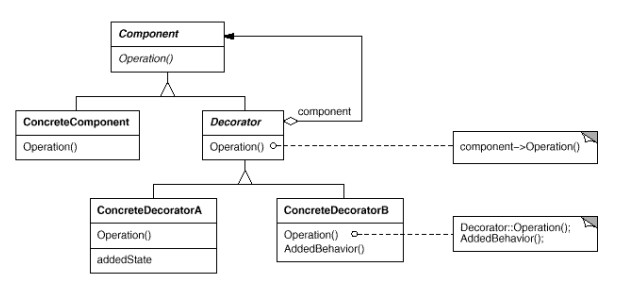
\includegraphics[scale=0.55]{imgs/decorator.jpg}
  \caption{Diagramma delle classi del pattern Decorator}
\end{figure}

\paragraph{Vantaggi}

Uno dei principali vantaggi del pattern è la flessibilità con cui permette di
aggiungere e rimuovere funzionalità a singoli oggetti a run-time. Inoltre, è
facile aggiungere più volte la stessa funzionalità (ad esempio, un bordo),
attribuendo due volte lo stesso decorator a un componente.

Il decorator permette di aggiungere gradualmente funzionialità agli oggetti:
invece che costruire classi grandi e complesse cercando di supportare più
funzionalità possibile, che potrebbero in futuro rivelarsi inutili, si possono
aggiungere incrementalmente solo quelle necessarie, definendo un nuovo Decorator
per ognuna di esse.

\paragraph{Svantaggi}

Un decorator e il componente incapsulato espongono la medesima interfaccia, ma
non sono identici. Non si può fare affidamento all'identità tra oggetti quando
vengono usati Decorator.

Un altro svantaggio sta nel fatto una progettazione basata su Decorator spesso
risulta in sistemi composti da molti piccoli oggetti simili tra loro. Essi
differiscono nel modo in cui sono interconnessi, ma non nelle classi di
appartenenza, e possono essere difficili da gestire in fase di debug.
